%# -*- coding: utf-8-unix -*-
%%==================================================
\chapter{设计模式}
\label{chap1}
\begin{itemize}[noitemsep,topsep=0pt,parsep=0pt,partopsep=0pt]
	\item ...
\end{itemize}

\section{知识点和方法论}
\subsubsection{多线程下单例设计模式}
(1) 饿汉式不会出现安全问题, 懒汉式会出现(同时创建的时候会有问题, 两个线程). \par
(2) 懒汉式安全隐患解决 \par
(3) 饿汉式, 在静态属性中就获取了对象, 懒汉式是去得到对象的时候获取, 导致了懒汉式可能有问题.
\begin{lstlisting}
package com.lf.shejimoshi;

/**
* @classDesc: 类描述:(懒汉式单例测试类) 
* @author baobaolan
* @createTime 2018年1月10日  
* @version v1.0
*/
public class SingletonTest {
	/**
	* @functionDesc: 功能描述:(测试懒汉式单例模式) 
	* @author baobaolan
	* @createTime 2018年1月10日  
	* @version v1.0
	*/
	public static void main(String[] args) {
		Student s1 = Student.getStudent();
		Student s2 = Student.getStudent();
		System.out.println(s1==s2);
	}    
	
}

/**
* @classDesc: 类描述:(学生类) 
* @author baobaolan
* @createTime 2018年1月10日  
* @version v1.0
*/
class Student{
	
	//定义全局变量
	private static Student student;
	
	//私有化构造函数
	private Student(){
		
	}
	
	/**
	* @functionDesc: 功能描述:(对外暴露方法) 
	* @author baobaolan
	* @createTime 2018年1月10日  
	* @version v1.0
	*/
	public static Student getStudent(){
		if(student==null){
			//加上同步锁,保证线程安全
			synchronized(Student.class){
				student = new Student();
			}
		}
		return student;
	}
}
\end{lstlisting}
\begin{lstlisting}
package com.lf.shejimoshi;

/**
* @classDesc: 类描述:(测试类) 
* @author baobaolan
* @createTime 2018年1月10日  
* @version v1.0
*/
public class Singleton2Test {
	
	public static void main(String[] args) {
		
		Teacher teacher1 = Teacher.getTeacher();
		Teacher teacher2 = Teacher.getTeacher();
		System.out.println(teacher1==teacher2);
		
	}
	
}

/**
* @classDesc: 类描述:(饿汉式单例) 
* @author baobaolan
* @createTime 2018年1月10日  
* @version v1.0
*/
class Teacher{
	//类加载的时候初始化一次
	private static final Teacher teacher = new Teacher();
	//私有化构造函数
	private Teacher(){
		super();
	}
	/**
	* @functionDesc: 功能描述:(对外暴露的方法) 
	* @author baobaolan
	* @createTime 2018年1月10日  
	* @version v1.0
	*/
	public static Teacher getTeacher(){
		return teacher;
	}
	
}
\end{lstlisting}
\subsubsection{为什么在wait代码块中要用while而不用if}
因为单个生产者单个消费者, 没什么问题. 如果是一个生产者两个消费者的话会有问题. \par
因为线程唤醒的话, 会直接在wait() 下面执行, 然后如果是while的话, 可以进入重新判断. 否则可能造成数据溢出. \par
\begin{lstlisting}
/*
生产和消费
*/
package multiThread;

class SynStack 
{
	private char[] data = new char[6];
	private int cnt = 0; //表示数组有效元素的个数
	
	public synchronized void push(char ch)
	{
		if (cnt >= data.length)
		{
			try
			{
				System.out.println("生产线程"+Thread.currentThread().getName()+"准备休眠");
				this.wait();
				System.out.println("生产线程"+Thread.currentThread().getName()+"休眠结束了");
			}
			catch (Exception e)
			{
				e.printStackTrace();
			}
		}
		this.notify(); 
		data[cnt] = ch;
		++cnt;
		System.out.printf("生产线程"+Thread.currentThread().getName()+"正在生产第%d个产品,该产品是: %c\n", cnt, ch);
	}
	
	public synchronized char pop()
	{
		char ch;
		if (cnt <= 0)
		{
			try
			{
				System.out.println("消费线程"+Thread.currentThread().getName()+"准备休眠");
				this.wait();
				System.out.println("消费线程"+Thread.currentThread().getName()+"休眠结束了");
			}
			catch (Exception e)
			{
				e.printStackTrace();
			}
		}
		this.notify();
		ch = data[cnt-1];
		System.out.printf("消费线程"+Thread.currentThread().getName()+"正在消费第%d个产品,该产品是: %c\n", cnt, ch);
		--cnt;
		return ch;        
	}    
}

class Producer implements Runnable
{
	private SynStack ss = null;
	public Producer(SynStack ss)
	{
		this.ss = ss;
	}
	
	public void run()
	{
		char ch;
		for (int i=0; i<10; ++i)
		{

			ch = (char)('a'+i);
			ss.push(ch);
		}
	}
}

class Consumer implements Runnable
{
	private SynStack ss = null;
	
	public Consumer(SynStack ss)
	{
		this.ss = ss;
	}
	
	public void run()
	{
		for (int i=0; i<10; ++i)
		{
			/*try{
				Thread.sleep(100);
			}
			catch (Exception e){            
			}*/
			
			//System.out.printf("%c\n", ss.pop());
			ss.pop();
		}
	}
}


public class TestPC2
{
	public static void main(String[] args)
	{
		SynStack ss = new SynStack();
		Producer p = new Producer(ss);
		Consumer c = new Consumer(ss);
		
		
		Thread t1 = new Thread(p);
		t1.setName("1号");
		t1.start();
		/*Thread t2 = new Thread(p);
		t2.setName("2号");
		t2.start();*/
		
		Thread t6 = new Thread(c);
		t6.setName("6号");
		t6.start();
		Thread t7 = new Thread(c);
		t7.setName("7号");
		t7.start();
	}
}
\end{lstlisting}
\subsubsection{Serializable}
序列化接口, 只有实现这个接口才能序列化, 默认计算一个serialVersionUID, 可以进行自定义.


\subsubsection{工厂模式}
\textbf{简单工厂模式}

简单来说就是使用字符串返回对象
\begin{figure}
	\centering
	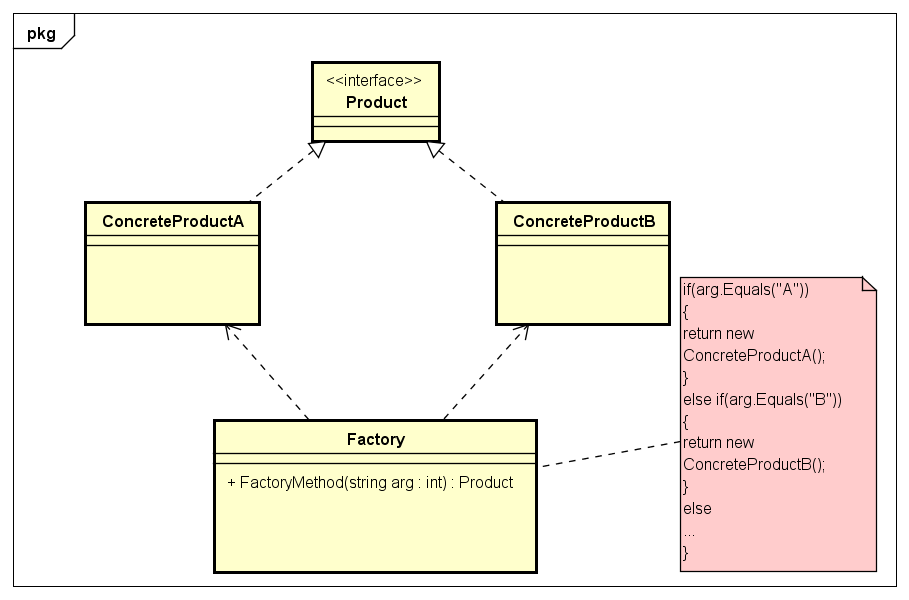
\includegraphics[width=0.7\linewidth]{figures/simpleFactory.png}
	\caption{simpleFactory}
	\label{fig:simpleFactory}
\end{figure}

\textbf{抽象工厂模式}

简单来说,就是工厂也是抽象化的, 原先只有产品是抽象化的

抽象工厂模式的优点
分离接口和实现
客户端使用抽象工厂来创建需要的对象,而客户端根本就不知道具体的实现是谁,客户端只是面向产品的接口编程而已。也就是说,客户端从具体的产品实现中解耦。

使切换产品族变得容易
因为一个具体的工厂实现代表的是一个产品族,比如上面例子的从Intel系列到AMD系列只需要切换一下具体工厂。

抽象工厂模式的缺点
不太容易扩展新的产品
如果需要给整个产品族添加一个新的产品,那么就需要修改抽象工厂,这样就会导致修改所有的工厂实现类。

\begin{figure}
	\centering
	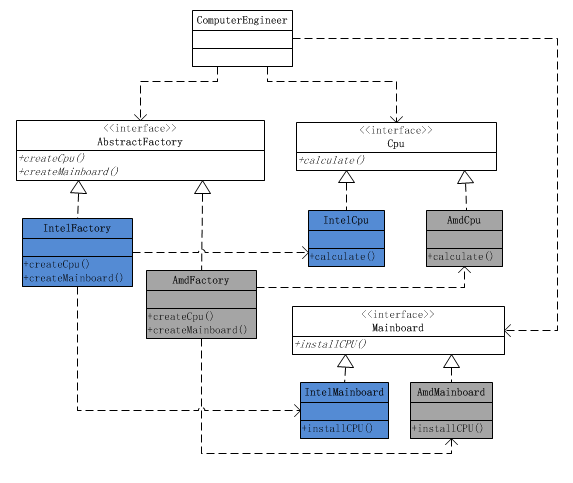
\includegraphics[width=0.7\linewidth]{figures/abstractFactory.png}
	\caption{abstractFactory}
	\label{fig:abstractFactory}
\end{figure}

\subsubsection{单例模式}
特点

1、单例类只能有一个实例。
2、单例类必须自己创建自己的唯一实例。
3、单例类必须给所有其他对象提供这一实例。

饿汉式(线程安全,调用效率高,但是不能延时加载):
\begin{lstlisting}
public class ImageLoader{ 
	private static ImageLoader instance = new ImageLoader; 
	private ImageLoader(){} 
	public static ImageLoader getInstance(){  
		return instance;  
	} 
}
\end{lstlisting}

DCL也就是双重锁判断机制(由于JVM底层模型原因,偶尔会出问题,不建议使用)
\begin{lstlisting}
public class SingletonDemo5 {
	private volatile static SingletonDemo5 SingletonDemo5;
	
	private SingletonDemo5() {
	}
	
	public static SingletonDemo5 newInstance() {
		if (SingletonDemo5 == null) {
			synchronized (SingletonDemo5.class) {
				if (SingletonDemo5 == null) {
					SingletonDemo5 = new SingletonDemo5();
				}
			}
		}
		return SingletonDemo5;
	}
}
\end{lstlisting}


\subsubsection{中介模式}



\subsubsection{代理模式}

分为静态代理和动态代理

现在可以看到,代理模式可以在不修改被代理对象的基础上,通过扩展代理类,进行一些功能的附加与增强。值得注意的是,代理类和被代理类应该共同实现一个接口,或者是共同继承某个类。

上面介绍的是静态代理的内容,为什么叫做静态呢?因为它的类型是事先预定好的,比如上面代码中的 Cinema 这个类。下面要介绍的内容就是动态代理。

\begin{lstlisting}
abstract class Move{
	public abstract void play();
}

class RealMove extends Move{
	public void play(){
		System.out.println("您正在观看电影 《肖申克的救赎》");
	}
}

class Cinema extends Move {
	RealMove movie;
	public Cinema(RealMove movie) {
		super();
		this.movie = movie;
	}
	
	
	@Override
	public void play() {
		guanggao(true);
		movie.play();
		guanggao(false);
	}
	
	public void guanggao(boolean isStart){
		if ( isStart ) {
			System.out.println("电影马上开始了,爆米花、可乐、口香糖9.8折,快来买啊!");
		} else {
			System.out.println("电影马上结束了,爆米花、可乐、口香糖9.8折,买回家吃吧!");
		}
	}
}


class ProxyTest {
	public static void main(String[] args) {
		RealMove realmovie = new RealMove();
		Move movie = new Cinema(realmovie);
		movie.play();
	}
}
\end{lstlisting}

\begin{lstlisting}
interface SellWine {
	void mainJiu();
}

class MaotaiJiu implements  SellWine{
	public void mainJiu(){
		System.out.println("我卖得是茅台酒");
	}
}

/*
* public static Object newProxyInstance(ClassLoader loader,
Class<?>[] interfaces,
InvocationHandler h)
loader 自然是类加载器
interfaces 代码要用来代理的接口
h 一个 InvocationHandler 对象
InvocationHandler 是一个接口,官方文档解释说,每个代理的实例都有一个与之关联的
InvocationHandler 实现类,如果代理的方法被调用,
那么代理便会通知和转发给内部的 InvocationHandler 实现类,由它决定处理。
InvocationHandler 内部只是一个 invoke() 方法,正是这个方法决定了怎么样处理代理传递过来的方法调用。
proxy 代理对象
method 代理对象调用的方法
args 调用的方法中的参数
* */

class GuitaiA implements InvocationHandler {
	private Object pingpai;
	
	public GuitaiA(Object pingpai){
		this.pingpai = pingpai;
	}
	
	public Object invoke(Object proxy, Method method, Object[] args) throws Throwable{
		System.out.println("销售开始  柜台是: "+this.getClass().getSimpleName());
		method.invoke(pingpai, args);
		System.out.println("销售结束");
		return null;
	}
}

class TestProxy{
	public static void main(String[] args) {
		MaotaiJiu maotaiJiu = new MaotaiJiu();
		InvocationHandler jinxiao1 = new GuitaiA(maotaiJiu);
		SellWine dynamicProxy = (SellWine) Proxy.newProxyInstance(MaotaiJiu.class.getClassLoader(),
		MaotaiJiu.class.getInterfaces(), jinxiao1);
		
		dynamicProxy.mainJiu();
	}
}
\end{lstlisting}


代理分为静态代理和动态代理两种。

静态代理,代理类需要自己编写代码写成。

动态代理,代理类通过 Proxy.newInstance() 方法生成。

不管是静态代理还是动态代理,代理与被代理者都要实现两样接口,它们的实质是面向接口编程。

静态代理和动态代理的区别是在于要不要开发者自己定义 Proxy 类。

动态代理通过 Proxy 动态生成 proxy class,但是它也指定了一个 InvocationHandler 的实现类。

代理模式本质上的目的是为了增强现有代码的功能。

Java动态代理只能代理接口,要代理类需要使用第三方的CLIGB等类库。

(动态代理优点)
传统面向对象思想中,如果想要实现功能复用,要么继承、要么引用,无论哪种方式,对代码都有一定的侵入性,耦合无可避免,侵入性啥意思?简单来说:如果你想要用它增强你程序的功能,你必须改动你的程序代码,那它就具有侵入性。如果只有一点两点需要增强还好说,如果大量的功能点需要被增强,工作量就会很大,代码也不太优雅。想象一下,如果你对外公开了一系列的接口,现在领导说了,接口要加权限控制。在哪加?最笨的当然就是写个程序验证的逻辑,然后每个接口都拿来调用一遍。这也正是面向对象思想的短板,在要为程序新增一些通用功能时,只能通过耦合的方式才能进行。AOP正是为此而生,AOP旨在通过一种无耦合的方式来为程序带来增强。而动态代理,就是AOP实现方式中的一种, 第2点决定了代理类需要把被代理类耦合进来,这意味着什么呢,代理类跟一个固定的被代理类绑定死了,如果你要对一百个类进行代理,即使代理逻辑一样,你也得编写一百个代理类(静态代理).


至此,Cglib动态代理的原理我们就基本搞清楚了,代码细节有兴趣可以再研究下。
最后我们总结一下JDK动态代理和Gglib动态代理的区别:

1.JDK动态代理是实现了被代理对象的接口,Cglib是继承了被代理对象。

2.JDK和Cglib都是在运行期生成字节码,JDK是直接写Class字节码,Cglib使用ASM框架写Class字节码,Cglib代理实现更复杂,生成代理类比JDK效率低。

3.JDK调用代理方法,是通过反射机制调用,Cglib是通过FastClass机制直接调用方法,Cglib执行效率更高。